% MA211 - Lecture 21
\documentclass[pdftex, xcolor=pdftex, dvipsnames,handout]{beamer}

\usetheme{MA211}
\usepackage{thumbpdf}
\usepackage{wasysym}
%\usepackage{ucs}
\usepackage[utf8]{inputenc}
\usepackage{pgf,pgfarrows,pgfnodes,pgfautomata,pgfheaps,pgfshade}
\usepackage{verbatim}

\usepackage{eurosym}
\usepackage{euler}

\usepackage{calc}               % Simple computations with LaTeX variables
%\usepackage[hang]{caption2}     % Improved captions

\usepackage{graphicx}           % Standard graphics package

\usepackage{amsmath, amsthm, amssymb}


\newcommand{\fquad}{\mbox{\qquad}}
\newcommand{\bull}{$\bullet$ }

\newcommand {\I} {\mathcal I}
\newcommand {\calI} {\mathcal I}
\def\disint{\displaystyle\int}

\DeclareMathOperator{\D}{d}
\newcommand{\dydx}{\frac{\D y}{\D x}}

%\definecolor{gray}{rgb}{0.69, 0.69, 0.69} \newcommand{\gray}[1]{\textcolor{gray}{#1}}
\definecolor{dogreen}{rgb}{0.33, 0.42, 0.18} \newcommand{\dogreen}[1]{\textcolor{dogreen}{#1}}
\definecolor{maroon}{rgb}{.5,0.2,0.2}\newcommand{\maroon}[1]{\textcolor{maroon}{#1}}
\definecolor{greena}{rgb}{.1,0.581,0.1}\newcommand{\greena}[1]{\textcolor{greena}{#1}}

\definecolor{blue4}{rgb}{0,0,.545}
\newcommand{\Blue}[1]{\textcolor{blue}{#1}}
\newcommand{\Red}[1]{\textcolor{red}{#1}}
\definecolor{pink}{rgb}{1.,0.75,0.8}
\definecolor{darkred}{rgb}{0.5,0.0,0.0}
\definecolor{darkgreen}{rgb}{0,0.3,0.3}
\definecolor{purple}{rgb}{0,0.3,0.3}
\definecolor{darkblue}{rgb}{0.0, 0.0, .5}
\definecolor{dpurple}{rgb}{.3,.0,.3}
\newcommand{\Green}[1]{\textcolor{darkgreen}{#1}}
\newcommand{\DRed}[1]{\textcolor{darkred}{#1}}
\newcommand{\DBlue}[1]{\textcolor{darkblue}{#1}}
\newcommand{\Purple}[1]{\textcolor{dpurple}{#1}}
\newcommand{\Emph}[1]{\textcolor{darkred}{\textbf{\it #1}}}
\newcommand{\remph}[1]{\textcolor{darkred}{\textbf{\emph{#1}}}}
\newcommand{\bemph}[1]{\textcolor{darkblue}{\textbf{\emph{#1}}}}
\newcommand{\gemph}[1]{\textcolor{darkgreen}{\textbf{\emph{#1}}}}
\newcommand{\Bf}[1]{\textcolor{darkblue}{\textbf{#1}}}
\newcommand{\Gf}[1]{\textcolor{darkgreen}{\textbf{#1}}}
\newcommand{\Rf}[1]{\textcolor{red}{\textbf{#1}}}
\newcommand{\Rmf}[1]{\textcolor{red}{\mathbf{#1}}}

\newcommand{\Conj}[1]{\overline{#1}}

\newcommand{\code}[1]{\textcolor{darkblue}{\texttt{\textbf{#1}}}}
\newcommand{\icode}[1]{{\blue\texttt{\textbf{\emph{#1}}}}}
\newcommand{\gcode}[1]{{\Green{\texttt{\textbf{\emph{#1}}}}}}
\newcommand{\out}[1]{\texttt{\emph{\textbf{\Green{#1}}}}}





\newenvironment{vminipage}%
{\begin{Sbox}\begin{minipage}\begin{small}\begin{verbatim}}%
{\end{verbatim}\end{small}\end{minipage}\end{Sbox}\fbox{\TheSbox}}

\newenvironment{nminipage}%
{\begin{Sbox}\begin{minipage}}%
{\end{minipage}\end{Sbox}\fbox{\TheSbox}}


\let\Arg\relax\DeclareMathOperator{\Arg}{\mathtt{Arg}}
\let\Arg\relax\DeclareMathOperator{\e}{\mathtt{e}}

\newcommand {\AND} {\wedge}
\newcommand {\OR} {\vee}
\newcommand {\NOT} {\neg}
\newcommand {\IMPLIES} {\rightarrow}
%\newcommand {\IFF} {\leftrightarrow}
\renewcommand {\iff} {\Leftrightarrow}
\newcommand {\NAND} {\uparrow}
\newcommand {\NOR} {\downarrow}
\newcommand {\XOR} {\otimes}

\newenvironment{citemize}% Colour items
{\begin{description}}%
{\end{description}}

\newcommand {\maroonitem}{\item[\maroon{$\bullet$}]}

\newcommand {\gitem} {\item {\includegraphics[width=.4cm,angle=-10]{img/green-bullet-on-white.ps}}}
\newcommand {\ritem} {\item {\includegraphics[width=.4cm,angle=-10]{img/red-bullet-on-white.ps}}}
\newcommand {\yitem} {\item {\includegraphics[width=.4cm,angle=-10]{img/yellow-bullet-on-white.ps}}}
\newcommand {\bitem} {\item {\includegraphics[width=.4cm,angle=-10]{img/blue-bullet-on-white.ps}}}

\newcommand {\greenitem} {\item {\includegraphics[width=.4cm,angle=-10]{img/green-bullet-on-white.ps}}}
\newcommand {\reditem} {\item {\includegraphics[width=.4cm,angle=-10]{img/red-bullet-on-white.ps}}}
\newcommand {\yellowitem} {\item {\includegraphics[width=.4cm,angle=-10]{img/yellow-bullet-on-white.ps}}}
\newcommand {\blueitem} {\item {\includegraphics[width=.4cm,angle=-10]{img/blue-bullet-on-white.ps}}}

\newcommand {\eq}[1]%
  {$\DBlue{#1}$}
\newcommand {\eqd}[1]%
  {$\displaystyle\DBlue{#1}$}
%\newcommand{\eq}[1]{\boldmath \DBlue{$#1$}}


\newcommand {\csf}{\centerslidesfalse}
\newcommand {\cst}{\centerslidestrue}

\newcommand {\vecii}[2] {   \big(\begin{smallmatrix} #1 \\ #2 \end{smallmatrix}\big)}
\newcommand{\atwo}[2]{\left(\!\!\begin{array}{c} #1 \\ #2 \end{array}\!\!\right)}


\newcommand{\C}{\mathbb{C}}
\newcommand{\Q}{\mathbb{Q}}
\newcommand{\R}{\mathbb{R}}
\newcommand{\N}{\mathbb{N}}
\newcommand{\Z}{\protect\mathbb{Z}}  % protect for index.
\newcommand {\Rs}{ \mathbb{R}}
\newcommand {\Cs}{ \mathbb{C}}
\newcommand {\Rnn}{ \mathbb{R}^{n \times n}}
\newcommand {\Rn}{ \mathbb{R}^{n}}


\newcommand{\mblock}{%
\setbeamercolor*{block title}{bg=maroon,fg=white}
\setbeamercolor*{block body}{bg=white,fg=maroon}
}%

\newcommand{\bblock}{%
\setbeamercolor*{block title}{bg=Steel,fg=white}
\setbeamercolor*{block body}{bg=Mylightgray,fg=Steel}
}%

\newcommand{\gblock}{%
\setbeamercolor*{block title}{bg=Green,fg=white}
\setbeamercolor*{block body}{bg=Mylightgray,fg=darkgreen}
}%


\newcommand{\rblock}{%
\setbeamercolor*{block title}{bg=Red,fg=white}
\setbeamercolor*{block body}{bg=white,fg=Black}
}%

\def\disfrac{\displaystyle\frac}
\newcommand{\TakeNotes}{
\includegraphics[width=2cm]{TakeNote}}

\def\eps{\varepsilon}
\newcommand {\del}[2]{ {\frac{\partial #1}{\partial #2}}}
\newcommand {\x}[1]{x^{[#1]}}
\newcommand {\delx}{ {\frac{\partial}{\partial x}}}
\newcommand {\delt}{ {\frac{\partial}{\partial t}}}
\newcommand {\dely}{ {\frac{\partial}{\partial y}}}
\newcommand {\ith}{{(i)}}
\renewcommand {\vec}[1]{ {\boldsymbol{#1}}}
\newcommand {\Oh} {\mathcal O}
\newcommand {\Err} {\mathcal E}
%\newcommand {\th} {\mathrm{th}}
\DeclareMathOperator{\fl}{fl}
\DeclareMathOperator{\sign}{sign}
\DeclareMathOperator{\Cond}{Cond} 
\DeclareMathOperator{\cond}{cond}
\DeclareMathOperator{\diag}{diag} 
\DeclareMathOperator{\sym}{sym} 
\DeclareMathOperator{\Trace}{Trace}

\DeclareMathOperator{\E}{e}

\newcommand {\Rsym}{{ \mathbb{R}^{n \times n}_\mathrm{sym}}}

\newcommand {\st} {\mathrm{st}}
\newcommand {\nd} {\mathrm{nd}}


\parskip .25cm


\theoremstyle{definition}
\newtheorem{exercise}{Exercise}[section]
\newtheorem{method}{Method}[section]

\newcommand{\Header}[1]{\begin{center}{\Large \Bf{#1}}\end{center}}

\subtitle{MA211}
\title{Lecture 22: 1st Order Differential Equations (Part II)}

\author{Dr Niall Madden}

\date{\Large Monday $24^\mathrm{th}$ Nov 2008}


\begin{document}

\setcounter{framenumber}{-1}
\frame{

%\begin{columns}[c]
%\column{0.45\textwidth}
%\centering
%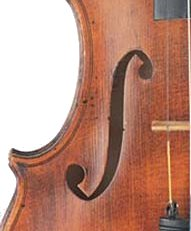
\includegraphics[width=4cm]{images/violin}
%
%
%\column{0.55\textwidth}
\begin{block}{}
\begin{center}
\begin{large}
 \insertsubtitle
\end{large}

\vspace{.1cm}

\begin{Large}
\textbf{\inserttitle}
\end{Large}


\vspace{.3cm}

{\insertdate}

\end{center}
\end{block}

\begin{center}
%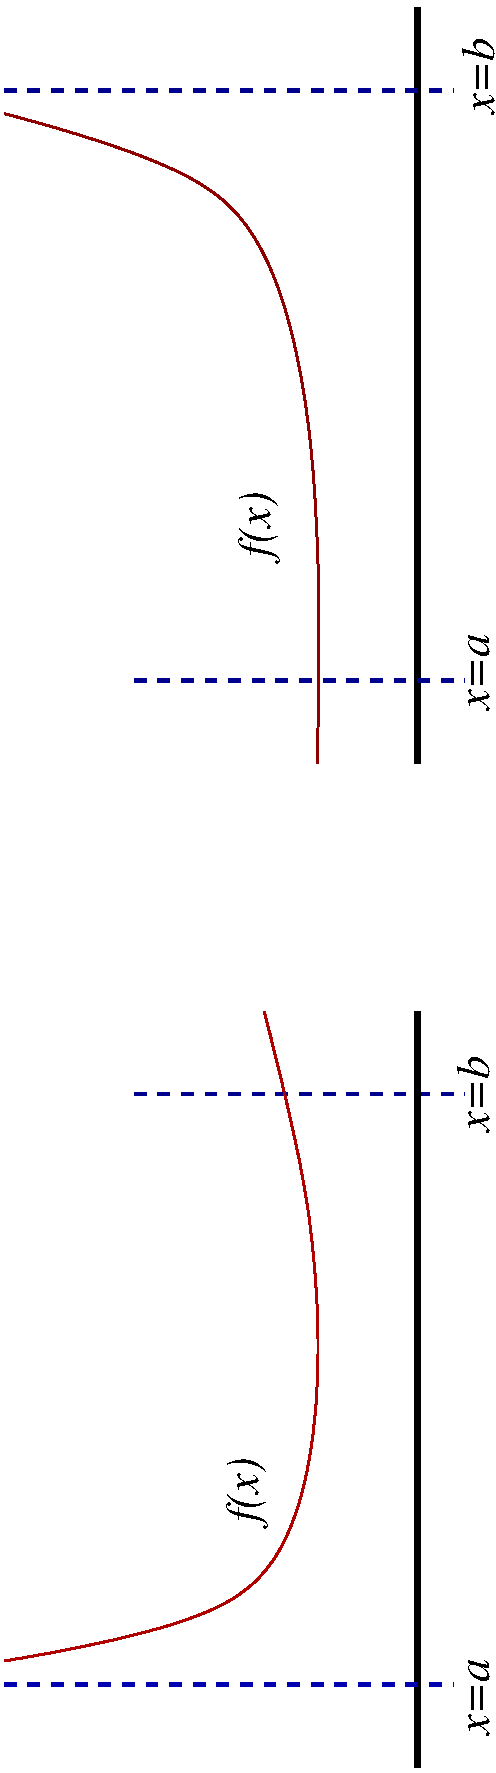
\includegraphics[width=3cm,angle=-90]{images/Improper2}
\end{center}


% \end{columns}

}

\frame{
  \frametitle{Topics of the day...}

%\begin{columns}[c]
%\column{0.5\textwidth}
 \tableofcontents
%\column{0.5\textwidth}


See also Sections 9.3 and 9.5 of Stewart.

%\end{columns}
}



\section{Recall: 1st Order Differential Equations}
\frame{

Last Wednesday, we started a new section on solving 1st order
differential equations.



\begin{block}{}
\begin{center}
\eqd{y'(x) = f(x,y)}.
\end{center}
\end{block}
}


%\section{Separable and Homogeneous 1st Order Equations}
\section{Recall: Separable  Equations}
\frame{


\begin{block}{}
A first order equation \eqd{\frac{dy}{dx} = f(x, y)} is \Bf{separable}
if we can write \eq{f(x)} as the product of some functions $g(x)$ and
$h(y)$. That is, it has the form 
\[
\frac{dy}{dx} =g(x)h(y).
\]
\pause
Such an equation can be solved by writing 
\[
\frac{1}{h(y)}dy = g(x)\,dx
\]
and integrating both sides:
\[
\int \frac{1}{h(y)}dy = \int g(x)\,dx
\]
\end{block}
}




\section{Recall: Homogeneous  Functions}
\frame{
Last Wednesday we also saw that 
a function \eq{f(x,y)} is \Bf{homogeneous} \Emph{of degree \eq{k}} if
for every real number \eq{t} we have 
\[
f(tx, ty) = t^k f(x,y).
\]


In interest to us is if right-hand side of the differential equation
$y'(x) = f(x,y)$ is  \emph{homogeneous of degree
  \eq{0}}. 

Then we can make the equation \Emph{separable} with the  substitution
\eqd{v = \frac{y}{x}}.

}




\section{Solving homogeneous DEs}
\frame{

Given a first order differential equation \eqd{\frac{dy}{dx}=f(x,y)}
where \eq{f(x,y}) is  \Emph{homogeneous of degree \alert{0}},

\begin{enumerate}
\item Let \eqd{v = \disfrac{y}{x}} and find the function \eq{h} such
  that
\eqd{ h(v) = f(x,y).}

\item  Because  we have \eqd{y=vx}, differentiate to get:
\eqd{\frac{dy}{dx} = v + x \frac{dv}{dx}}

\item Substitute into the original differential equation:\\
\qquad \eqd{ v + x\disfrac{dv}{dx} = h(v).}

\item This equation involving \eq{v} and \eq{x} is separable:
\[ \frac{1}{h(v)-v}dv=\frac{1}{x}dx\]

\item Solve it in the same way we solve the separable problems from
  last week.
\end{enumerate}
}

\frame{

\begin{example}
Solve the equation $\disfrac{dy}{dx}=\disfrac{xy+y^2}{x^2}$.
\end{example}

%\und{Solution}: $f(tx,ty) = f(x,y)$ so \eq{f} is homogeneous of degree
%\alert{0}. \\
%3Write $v = \disfrac{y}{x}$. Then $\disfrac{dy}{dx} = v +
%x\disfrac{dv}{dx}$ and 
%$$
%v + x\disfrac{dv}{dx} = v+v^2\Longrightarrow x\disfrac{dv}{dx} = v^2.
%$$
%Thus 
%$$
%\frac{1}{v^2}\,dv = \frac{1}{x}\,dx\Longrightarrow
%\int\frac{1}{v^2}\,dv = \int\frac{1}{x}\,dx.
%$$
%Hence 
%$$
%-\frac{1}{v} = \ln |x|+C\Longrightarrow v = \frac{y}{x} =
%\frac{-1}{\ln |x|+C}.
%$$
%Solution : $y = \disfrac{-x}{\ln |x|+C}$. 

\vspace{3cm}

}

\frame{
\begin{example}
Solve the following initial value problem:
\[ 
  \frac{dy}{dx} = \disfrac{x^2 + xy}{xy + y^2}, \qquad y(2)=1.
\]
\end{example}
\vspace{4cm}
}

\frame{
\begin{example}[Autumn  exam 07/08, Q4(iii)]

Solve the following differential equation:
\[ 
  2xy \frac{dy}{dx} = x^2 + y^2, \qquad y(2)=2.
\]
\end{example}
\vspace{4cm}
}

\frame{
\begin{exercise}[22.1]
Find the general solution to the following differential equations:
\begin{enumerate}
\item \eqd{  \frac{dy}{dx} = \disfrac{x + y}{x - y}.}
\item \eqd{  \frac{dy}{dx} = \disfrac{xy}{x^2 +2y^2}.}
\end{enumerate}
\end{exercise}

\begin{exercise}[22.2]
Solve the following initial value problems:
\begin{enumerate}
\item \eqd{  \frac{dy}{dx} = \disfrac{x^2 + xy + y^2}{x^2}; \quad y(1)=1.}
\item \eqd{  \frac{dy}{dx} = \disfrac{x^3 + 3xy^2}{3x^2y + y^3};
    \qquad y(1)=-1}
\end{enumerate}
\end{exercise}

}




\section{First Order Linear Differential Equations}
\frame{

To finish the course, we'll look at ways of solving  \Emph{first order
  linear} differential equation such as:
\[
\frac{dy}{dx}+P(x)y = Q(x).
\]

This is called \Emph{Linear} because the only expression for \eq{y} is
linear.
}

\frame{
\begin{example}
These are linear equations:
\begin{itemize}
\item  \eqd{\frac{dy}{dx}-3y = e^x}. 
\item  \eqd{x \frac{dy}{dx} + y = \sin(x)}. 
\item  \eqd{ \frac{dy}{dx} + \sqrt{x} y = \ln(x)}. 
\end{itemize}

These are \Bf{not} linear:
\begin{itemize}
\item  \eqd{\frac{dy}{dx}- y^3 = e^x}. 
\item  \eqd{y \frac{dy}{dx}  = \sin(x)}. 
\item  \eqd{ \frac{dy}{dx} +  x \sqrt{y} = \ln(x)}. 
\end{itemize}
\end{example}
}

\frame{
A general strategy for solving such an equation is to multiply the
equation by  some expression \eq{v(x)} that simplifies the problem.
Then we get:
\[
v(x)\frac{dy}{dx} + v(x)P(x)y = v(x)Q(x).
\]
The idea is to choose \eq{v(x)} so that the left hand side of the above
equation is the derivative of the product \eq{vy}. This would require 
\[
v\frac{dy}{dx}+vP(x)y = v\frac{dy}{dx}+y\frac{dv}{dx},
\]
that is
\[
vP(x) y = y\frac{dv}{dx}\ \Longrightarrow \frac{dv}{dx}=vP(x).
\]
}
\section{Integrating Factors}

\frame{
So we need to choose $v$ so that $\disfrac{dv}{dx}=vP(x)$. This means:

\begin{block}{}
\vspace{4cm}
\end{block}


The expression \eq{v(x)} is called an \Emph{integrating factor} for the
differential equation. 
}

\frame{
\begin{example}
Solve the differential equation $y'-3y = e^x$. 
\end{example}
%\n\und{Solution}: Note this equation is not separable. \\
%This is a linear equation with $P(x)=-3,\ Q(x)=e^x$. \\
%Integrating factor $v(x) =e^{\int -3dx} = e^{-3x}$. 
%Multiplying the equation through by $v(x) = e^{-3x}$ gives 
%$$
%e^{-3x}\frac{dy}{dx}-3e^{-3x}y = e^{-3x}e^x = e^{-2x}.
%$$
%Thus 
%\begin{eqnarray*}
%\frac{d}{dx}(e^{-3x}y) = e^{-2x} & \Longrightarrow & e^{-3x}y =
%-\frac{1}{2}e^{-2x}+C \\
%y & = & -\frac{1}{2}e^x+Ce^{3x}.
%\end{eqnarray*}
\vspace{4.5cm}

}

\subsection{Technique}
\frame{

\Header{Summary of Technique of Integrating Factors}

Given a problem of the form:
\[
\frac{dy}{dx} + P(x)y = Q(x).
\]
\begin{enumerate}
\item Let  \eqd{v  = e^{\int P(x) dx}}.
\item Solve \eqd{(vy)' = v Q(x)} by integrating:
\[
vy = \int v Q(x) dx.
\]
not forgetting the constant of integration.

\item Divide by \eq{v} to get the solution:
\[
y = \frac{\int v Q(x) dx}{v}.
\]
\end{enumerate}
}

\subsection{Examples}
\frame{

\begin{example}
Solve the equation 
\[
x \disfrac{dy}{dx}+ y = \sin(x)
\]
subject to the initial condition $y(\pi /2) = 1$.
\end{example}

%\n\und{Solution}: $\disfrac{dy}{d\theta}+\disfrac{1}{\theta}y =
%\disfrac{1}{\theta}\sin\theta$. \\
%Integrating factor $v = e^{\int\frac{1}{\theta}\,d\theta} =
%e^{\ln\theta}=\theta$. 
%Then 
%\begin{eqnarray*}
%\theta\frac{dy}{d\theta} + y =\sin\theta & \Longrightarrow &
%\frac{d}{d\theta}(\theta y) = \sin\theta \\
%& \Longrightarrow & \theta y = -\cos\theta + C \\
%& \Longrightarrow & y(\theta) = \frac{-\cos\theta+C}{\theta} \\
%\end{eqnarray*}
%Now $y(\pi /2) = 1\Longrightarrow \disfrac{-0+C}{\pi
%/2}=1\Longrightarrow C=2/\pi$. Thus 
%$$
%y(\theta ) = -\frac{\cos\theta }{\theta}+\frac{\pi}{2\theta}.
%$$

\vspace{4cm}

}

\frame{

\begin{example}
Solve the equation 
$$
x\frac{dy}{dx}-y = x^3,\ \ y(1)=1.
$$
\end{example}
%\n\und{Solution}: $\disfrac{dy}{dx}+\left(-\disfrac{1}{x}\right)y =
%x^2$. \\
%Integrating factor $v(x) = e^{\int -1/x\,dx} = e^{-\ln x} =
%\disfrac{1}{x}$.
%Then 
%\begin{eqnarray*}
%\frac{1}{x}\frac{dy}{dx}-\frac{1}{x^2}y = x^2 & \Longrightarrow & 
%\frac{d}{dx}\left(\frac{y}{x}\right) = x^2 \\
%& \Longrightarrow & 
%\frac{y}{x} = \frac{x^3}{3}+C \\
%& \Longrightarrow & 
%y = \frac{x^4}{3}+Cx. 
%\end{eqnarray*}
%Now $y(1)=1\Longrightarrow \disfrac{1}{3}+C = 1,\ C =
%\disfrac{2}{3}$. \\
%Solution $y = \disfrac{x^4}{3}+\disfrac{2x}{3}$. 

\vspace{4cm}
}



\frame{
\begin{example}[Q3(c), Semester 1, '06/'07]
\[ e^x\frac{dy}{dx} + 2e^x y = 1.\]
\end{example}

\vspace{5cm}
}


\frame{
\begin{example}
Solve the following differential equation:
\[ 
\frac{dy}{dx} + \cos(x) y = 2xe^{-\sin(x)}.
\]
\end{example}

\vspace{5cm}
}


\frame{
\begin{exercise}
Solve the following differential equations:
\begin{enumerate}[(i)]
\item \eqd{y' + \frac{y}{x} = x^2 - \frac{1}{x}, \qquad y(1)=1/4.}
\item \eqd{y' + 2y = e^{-x}.}
\item \eqd{y' = x^2 + x^2y}
\item \eqd{y' + 3xy =x}
\item \eqd{y' = \sin(x)y = 3\sin(2x)}
\item \eqd{xy' + y = 2x \sin(x)}
\item \eqd{2xyy' =x^2 +3y^2}
\item \eqd{y' + \frac{y}{\tan(x)} = 3x+1}

\end{enumerate}
See also: Problem Set 5.
\end{exercise}
}
\end{document}


